\documentclass{report}

\input{~/latex/template/preamble.tex}
\input{~/latex/template/macros.tex}

\title{\Huge{Chapter 6 Lecture Notes  }}
\author{\huge{Matt Warner}}
\date{\huge{}}
\pagestyle{fancy}
\fancyhf{}
\rhead{}
\lhead{\leftmark}
\cfoot{\thepage}
% \usepackage[default]{sourcecodepro}
% \usepackage[T1]{fontenc}
\usepgfplotslibrary{fillbetween}


\pgfpagesdeclarelayout{boxed}
{
  \edef\pgfpageoptionborder{0pt}
}
{
  \pgfpagesphysicalpageoptions
  {
    logical pages=1,%
  }
  \pgfpageslogicalpageoptions{1}
  {
    border code=\pgfsetlinewidth{1.5pt}\pgfstroke,%
    border shrink=\pgfpageoptionborder,%
    resized width=.95\pgfphysicalwidth,%
    resized height=.95\pgfphysicalheight,%
    center=\pgfpoint{.5\pgfphysicalwidth}{.5\pgfphysicalheight}%
  }%
}

\pgfpagesuselayout{boxed}

\begin{document}
  \maketitle
  \section*{6.1 Probability Distributions for a Continuous Random Variable}
  \bigbreak \noindent
  \subsection*{2 Types of Random Variables}
  \begin{itemize}[label=$\bullet$]
    \item \textbf{Discrete} 
      \begin{itemize}[label=$\circ$]
        \item \textbf{possible values} -  a finite set or a countably infinite set \\ (usually associated with counting, e.g. ``the number of...'')
      \bigbreak \noindent
        \item \textbf{Probability distribution} - specified by giving a
          \begin{itemize}[label=$\circ$]
            \vspace{1em}

          \item Table  
            \vspace{5mm}
            \begin{center}
            \begin{tabular}{c|cccccc}
            $x$ & 1 & 2 & 3 & 4 & 5 & 6 \\
            \hline$p(x)$ & 0.40 & 0.20 & 0.12 & 0.10 & 0.14 & 0.04
            \end{tabular}
            \end{center}
            \bigbreak \noindent
            \vspace{2mm}

            \item Probability Mass Function
              $$ e.g. \ \  p(x) = {n \choose x} \cdot p^x \cdot (1 - p)^{n-x} \hspace{5mm} \text{for x = 0,1,2..., n}$$
            \bigbreak \noindent
          \item \textbf{Example} - Binomial distribution
          \end{itemize}
      \end{itemize}
      \bigbreak \noindent
    \item \textbf{Continuous}
      \begin{itemize}[label=$\circ$]
        \vspace{1em}

        \item \textbf{Possible values} - an infinite set that forms an interval on the number line \\ (usually associated with measuring, e.g. heights, weights, volumes, times, etc.)
          \bigbreak \noindent
        \item \textbf{Probability distribution} - specified by giving a \textbf{probability density function}
          \bigbreak \noindent
        \item \textbf{Example} - Normal distribution
      \end{itemize}
  \end{itemize}
  \bigbreak \noindent \bigbreak \noindent
  \hrule
  \subsection*{Probability Density Function}
  \bigbreak \noindent
  \begin{minipage}{0.45\textwidth}
    \vspace{-10mm}A Probability Density Function is a curve that 
  \begin{itemize}
    \item Is on or above the x-axis
    \item Has total area = 1.0
  \end{itemize}
  \end{minipage}
  \hspace{2em}\begin{minipage}{0.4\textwidth}
    \incfig[1]{brr}
  \end{minipage}

\bigbreak \noindent
\pagebreak
\subsection*{The Normal Distribution}
\begin{itemize}
  \item The \textbf{Normal Distribution} is defined by a probability density function that is a symmetric, bell shaped curve.
    \bigbreak \noindent
  \item It is used to suggest or hypothesize a distribution for an \textbf{\textit{entire population}}
    \bigbreak \noindent
  \item There are many normal distributions. Each is identified by giving values of
    \bigbreak \noindent
    \begin{itemize}[label=$\circ$]
      \item $\mu$ = \underline{population mean}  \hspace{11em} (Note $\bar{x}$ = \underline{sample mean}) 
      \bigbreak \noindent
    \item $\sigma$ = \underline{population standard deviation} \hspace{5em} (Note: s = \underline{sample}std. dev.)
    \end{itemize}
\end{itemize}
\bigbreak \noindent \bigbreak \noindent
\q 

    Sketch the normal distribution corresponding to each of the following
    \bigbreak \noindent
    a) $Z \(\sim\) N(\mu = 0, \sigma = 1)$
    \bigbreak \noindent
    \begin{center}
    \begin{tikzpicture}
  \begin{axis}[
    no markers, domain=-3:3, samples=100,
    axis lines=left, xlabel=$\mu$, 
    height=5cm, width=10cm,
  ]
  \addplot[black, thick] {1/(sqrt(2*pi))*exp(-x^2/2)};
  \end{axis}
\end{tikzpicture}
\end{center}

\bigbreak \noindent
    b) X \(\sim\) N($\mu = 5, \sigma = 1)$
\bigbreak \noindent
\begin{center}
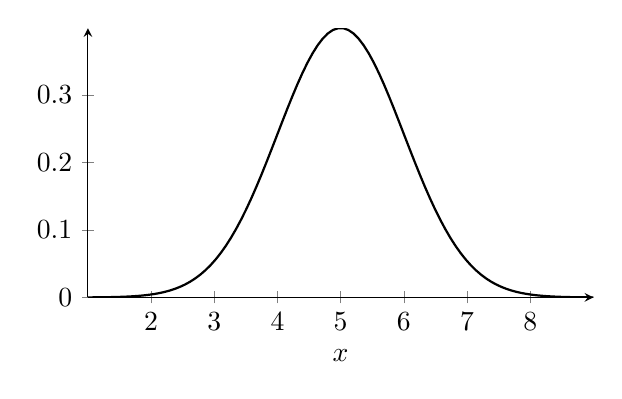
\begin{tikzpicture}
  \begin{axis}[
    no markers,
    domain=1:9,
    samples=100,
    axis lines=left,
    xlabel=$x$,
    height=5cm,
    width=8cm,
    xtick={2, 3, 4, 5, 6, 7, 8}, % Custom x-axis tick positions
  ]
    \addplot [black, thick] {1/(sqrt(2*pi)*1) * exp(-(x-5)^2/2)};
  \end{axis}
\end{tikzpicture}
\end{center}
\pagebreak
\nt{
  \begin{itemize}
    \item The Standard normal distribution is the most important one to  understand. 
    \item Any generic or \textbf{\underline{non-standard normal}} X\sim\)N($\mu,\sigma$) can be converted into the standard normal using the formula $Z = \dfrac{x -\mu}{\sigma}$
    \item Any desired probability about the random variable X is found by \textbf{\underline{standardizing X}} to produce Z and then using the table of standard normal cumulative probabilites (commonly called the \textbf{\underline{Z table}})
  \end{itemize}
}
\q
\bigbreak \noindent
Let the random variable X represent the SAT score of a randomly chosen student. Suppose that the SAT scores of all students in the population vary according to a normal distribution with mean $\mu$ = 1050 and standard deviation $\sigma$ = 150
\bigbreak \noindent
\textbf{What does the empirical Rule tell us about the following probabilities}
    
    \bigbreak \noindent
    a) $P(900 <X<1200) = .68 \rightarrow 1$ standard deviation from the mean
    \bigbreak \noindent
    b) $P(750 <X<1350)$ = .95 $\rightarrow$ 2 standard deviation from the mean
    \bigbreak \noindent
    c) $P(600<X<1500)$ = .997 $\rightarrow$ 3 standard deviation from the mean
    \bigbreak \noindent \bigbreak \noindent
    \hrule
    \bigbreak \noindent
    \textbf{Find the probability that a randomly selected student scores less than 1275}
    \bigbreak \noindent
    That is,

    $$P(X<1275)$$
To find this we can use the formula

$$ Z = \dfrac{x - \mu}{\sigma}$$
So, we get

    $$ Z = \dfrac{1275 -1050}{150}$$
So,

    $$ Z = 1.50 $$
Now we can find the the probability by using the Z table.
\bigbreak \noindent
$$ P(X < 1275) = .9394$$
\bigbreak \noindent
% \nt{
%   Since the question was specifically looking for the area to the left of x, our answer is the value corresponding to the Z score,
%   \bigbreak \noindent
%   If the question was looking for $X > 1275$, our answer would be 1 - .9394
% \bigbreak \noindent 
% \hline
% $$ P(X < x) = \text{value found directly from Z table}$$.
%
% $$ P(X > x) = \text{value found from 1 - value found in Z table}$$
%
% $$ P(x_1 < X < x_2) = \text{value found from }
%
% }
    \bigbreak \noindent
    \hrule
    \bigbreak \noindent
    \textbf{Find the probability that the student scores more than 800}
    \bigbreak \noindent
    That is,
    $$P(X>800)$$
    So,
    $$ P(\frac{x - 800}{150} > \frac{800 - 1050}{150})$$
    Now we have,
    $$ P(Z > -1.67)$$
    which gives us,
    $$ P(X > 800) =  0.0475$$

  \pagebreak
\bigbreak \noindent
\textbf{Find $\mathbf{P(1100 \le X \le 1270)}$}
\bigbreak \noindent
That is,

$$P(\frac{1100 - 1050}{150} \le Z \le \frac{1270 - 1050}{150})$$
Solving that leaves us with,

$$ P(.33 \le Z \le 1.47)$$

\bigbreak \noindent Lets get all the area to the left of 1.47

$$ P(Z = 1.47) = .9292$$
\bigbreak \noindent 
Now, lets get everything to the left of .33

$$P(Z = .33) = .6293$$
\bigbreak \noindent
Now, we subtract them
$$ .9292 - .6293 = \boxed{.2999}$$
\bigbreak \noindent
\hrule
\bigbreak \noindent
\textbf{25\% of students score \underline{less} than \_\_\_\_\_\_\_\_\_\_\_.}
\bigbreak \noindent
We need to find the Z score in the table find by finding the closest value to .25

$$ P(X < .25) = -.67$$
Using the equation

$$ Z = \dfrac{x - \mu}{\sigma}$$
We can solve for x

$$ -0.67 = \frac{x - 1050}{150}$$

$$ x = 949.5$$
\bigbreak \noindent
\hrule
\bigbreak \noindent
\textbf{The top 10\% of students score more than \_\_\_\_\_\_\_\_\_. }
\nt{
  This is the same as asking for the value b so that $P(X > b) = .10$, which could also be called the 90th percentile.
}
\bigbreak \noindent
Find the value in the table closest to .90

$$ Z = 1.28$$
using the formula for Z, we can find b, 

$$ 1.28= \frac{b - 1050}{150}$$
So,
$$ b = 1242.2$$
\bigbreak \noindent
Therefore, the top 10\% of students score more than 1242.2
\bigbreak \noindent
\textbf{find a symmetric interval about the mean that will capture the central 90\% of SAT scores. That is, find the values L and U (where L and U are equally distant from the mena), so that} $$P(L < X < U) = .90$$
\bigbreak \noindent
 If we are asked for the middle 90\%, then our left and right tails are both .05
\bigbreak \noindent
So our z scores are $\pm{1.6449}$
\bigbreak \noindent
Now we solve
$$ 1.6449 = \frac{u - 1050}{150} = 1296.7$$

$$ -1.6449 = \frac{l -1050}{150} = 808.3$$
So our interval is,
$$(1296.7, 808.3)$$
\bigbreak \noindent
\hrule
\bigbreak \noindent
\q
\bigbreak \noindent
\textbf{The virginia Cooperative Extension reports that the mean weight of yearling Angus steers is 1152 pounds. Suppose that weights of all such animals can be described by a Normal model with a standard deviation of 84 pounds}
\bigbreak \noindent
\centerline{\textbf{What percent of steers weigh}}
  \bigbreak \noindent
  \hrule
  \bigbreak \noindent
  \textbf{a) Less than 120 Pounds}
\bigbreak \noindent
  That is,

  $$P(X < 1200)$$
  So,

  $$ P(\frac{x-1152}{84} < \frac{1200 - 1152}{84})$$

  $$ P(Z < .57)$$
  \bigbreak \noindent
Now we look up the value 0.57 in the table to find the probability.
$$ P(Z < .57) = .7157$$
\bigbreak \noindent
\hrule
\bigbreak \noindent
\textbf{b) Less than 950 pounds}
\bigbreak \noindent
That is,
$$ P(X < 950)$$

\pagebreak
\noindent
\textbf{c) Greater than 1250 pounds}
\bigbreak \noindent
That is,

$$P(X > 1250)$$
So,

$$P(X > 1250) = \frac{1250- 1152}{84}$$
So we have,

$$ Z = 1.17$$
Looking in the table we find,

$$P(Z = 1.17) = .8790$$
Now we subtract 1 from that giving us,

$$P(X > 1250) = 1 - .8790$$
$$ = .1210$$
\bigbreak \noindent
\nt{
  Always round the Z scores to 2 decimal places
}
\end{document}
